\section{Recursión}
\begin{frame}[fragile]
  \frametitle{Recursión}
  {\color{white}
    \inputminted[bgcolor=bg]{haskell}{code/recursion01.hs}
  }
\end{frame}

\begin{frame}[fragile]
  \frametitle{Recursión}
  {\color{white}
    \inputminted[bgcolor=bg]{haskell}{code/recursion02.hs}
  }
  {\color{white}
    \inputminted[bgcolor=bg]{haskell}{code/recursion02.hs}
  }
\end{frame}


\begin{frame}
  \frametitle{Recursos adicionales}
  \begin{columns}
    \begin{column}{0.5\textwidth}
      \textbf{\textit{Learn You a Haskell for Great Good!}}\\
      \url{http://learnyouahaskell.com/chapters}
    \end{column}
    \begin{column}{0.5\textwidth}  %%<--- here
      \begin{center}
        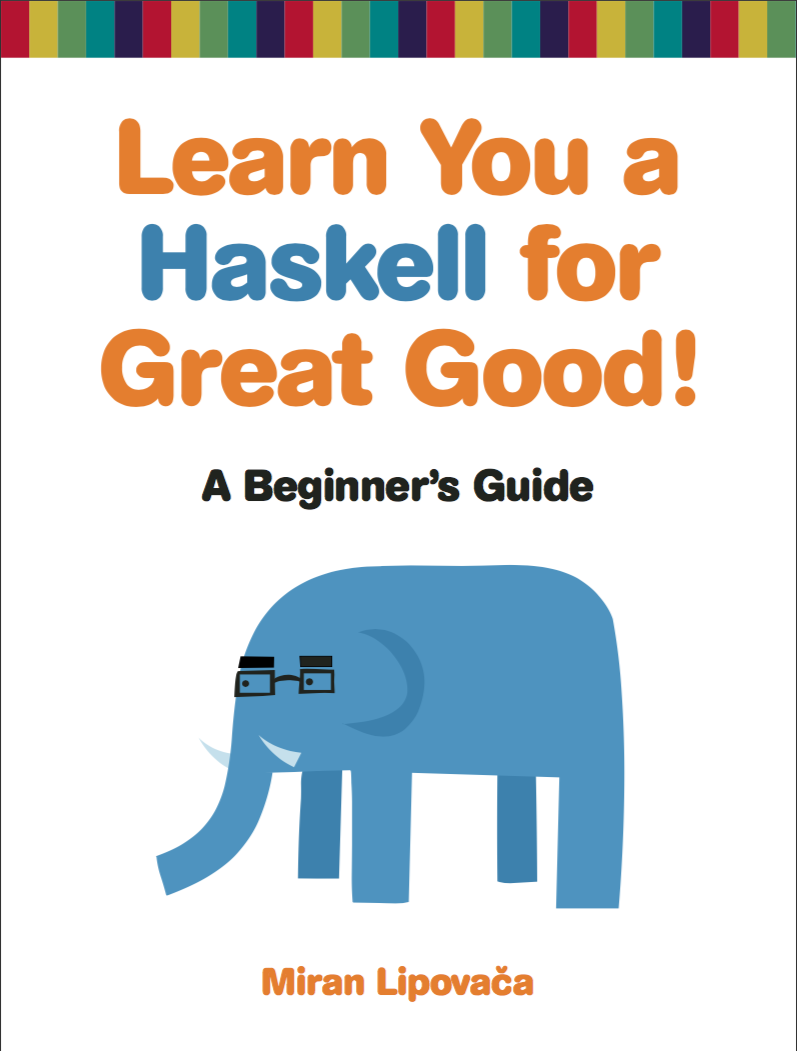
\includegraphics[width=0.5\textwidth]{img/LYH.png}
      \end{center}
    \end{column}
  \end{columns}
\end{frame}

% \begin{frame}
%   \frametitle{Recursos para continuar}
%   \begin{columns}
%     \textbf{Learn You a Haskell for Great Good!}
%     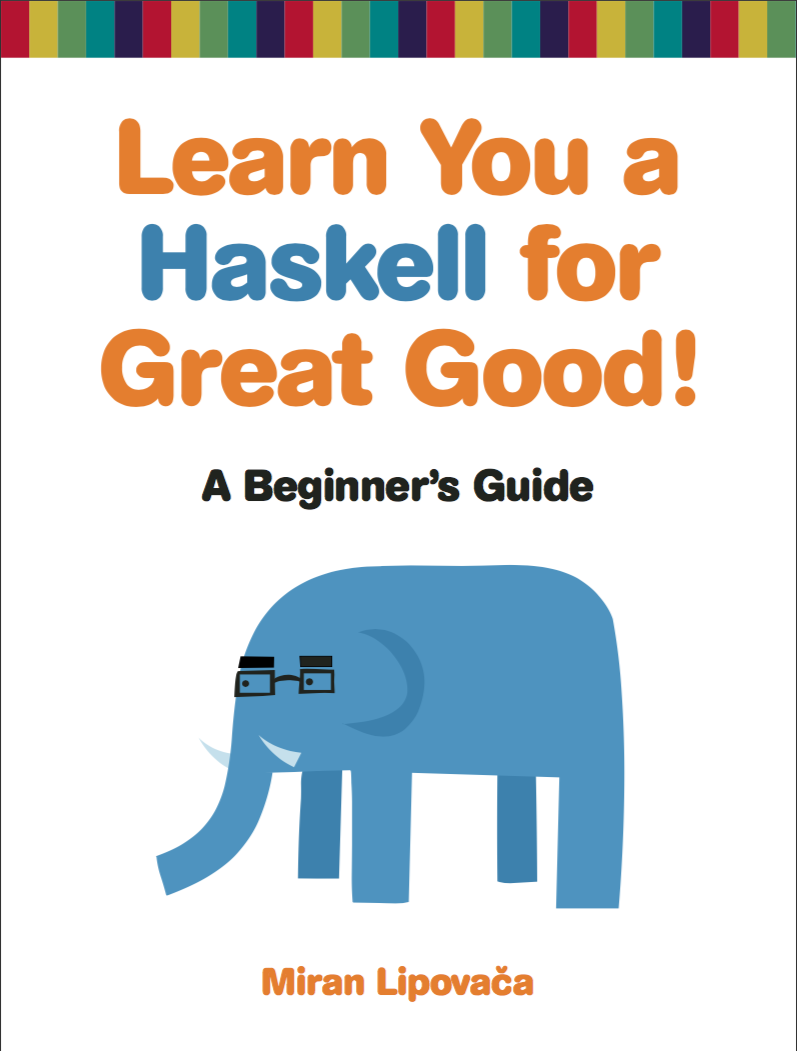
\includegraphics[width=0.5\textwidth]{img/LYH.png}
%   \end{column}
% \end{frame}